This subsection is meant to serve as a brief description of \cite{Escolar2016}. Refer to the original paper for more thorough descriptions (including pseudo code) or details regarding computational complexity. Suppose we have a $q$-cycle $z$ which we seek to minimize with respect to the 1 norm $\left|\left| \sum a_j\sigma_j \right|\right| = \sum |a_j|$ on the space $C_q(K) = \text{span}\{\sigma_j\}$, where $\sigma_j$ are $q$ simplices in $K$. A first approach to minimization could be to consider the linear optimization problem
\begin{align*}
    \text{minimize } & ||x||_1\\
    \text{subject to } & x - \partial_{q+1}y = z\\
    & x, y \text{ integral}
\end{align*}
where $\partial_{q+1}$ is the $q+1$st boundary matrix and $y$ is any $q+1$-chain. Essentially, this system of equations searches for a $q$-chain $x$ with minimal size which is homologous to our original cycle $z$. We call our minimal solution $x = \Tilde{z}$. Now instead, suppose we have a simplex-wise filtration $K_b$, where one simplex $\sigma_b$ is added at each filtration step. At any given filtration step, then, we gain at most one $q$-cycle. Call that $q$-cycle $z$ and call previous (known) cycles $\{g_j\}$ and consider the following problem, modified from above:
\begin{align*}
    \text{minimize } & ||x||_1\\
    \text{subject to } & x - \partial_{q + 1}y + \sum a_j g_j = z\\
    & x,y,a \text{ integral}
\end{align*}
We call our solution to this algorithm $\Tilde{z}_j$. Finally, if we let $\{\Tilde{z}_j\} = \{g_j\}$ be minimal cycles found at previous steps and perform the above algorithm, we find a minimal cycle at each step.

One observation regarding this algorithm is that it computes an optimal cycle $\Tilde{z}_j$ only once, then does not modify it. If, for example, the feature enclosed by $\Tilde{z}_j$ split into two holes, $\Tilde{z}_j$ would enclose both holes. Although this might not be considered ``optimal" at this step, modifying $\Tilde{z}_j$ at future steps would likely produce a cycle that does not exist for the entire time the feature persists.


Below is an example of the result of this algorithm, sampled from a noisy circle:
\begin{figure}[h]
    \centering
    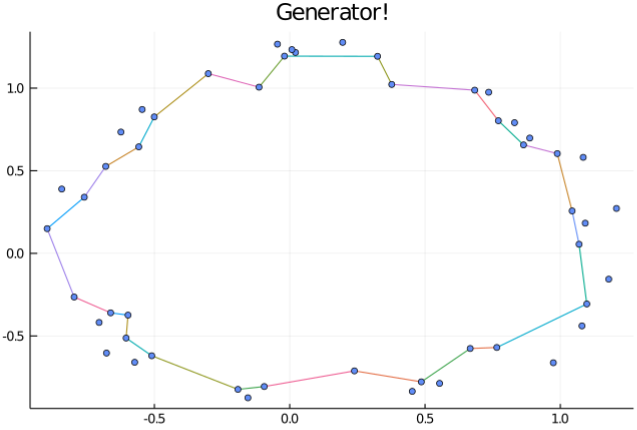
\includegraphics[width = .45\textwidth]{NoisyCircleOrig.png}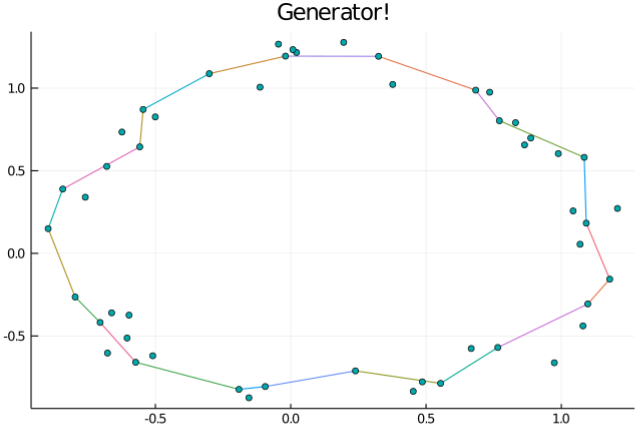
\includegraphics[width = .45\textwidth]{NoisyCircleMin.png}
    \caption{A generator found from our algorithm (left) and the minimal version of it (right) found via linear programming as described in \cite{Escolar2016}}
    \label{EscolarMinGen}
\end{figure}
Note this cycle is not also volume-minimal: the original generator contains 28 1-simplices, and the minimal version contains 21, but the minimal version encloses a greater area. See a later section and \cite{Obayashi2018} for an algorithm which computes volume-optimal cycles. Also note that some modifications to the generator were unnecessary: around the (-.5,.75) coordinate the generator switches between one pair of 1-simplices and another, for no clear reason.




